\section{Búsqueda de contratos inteligentes similares}
\label{appendix:sim_code}

La dificultad en la búsqueda de similaridad de código radica en las características estructurales de los lenguajes de alto nivel, y en la diversidad de las expresiones lógicas de los contratos inteligentes. En la actualidad existen varias escuelas de algoritmos de búsqueda de similaridad de código en los círculos académicos, las que se describen de este modo:

\begin{itemize}
	\item \textbf{Distancia de edición entre cadenas de caracteres} \\
	Both of the entered query code and candidate source code are deemed as texts. Edit distance between two character strings is used for measuring similarity between them. Edit Distance refers to the minimum number of editing operations required for converting one character string into the other character string. Permitted editing operations include replacement of one character with another character, i.e. insertion of a character and deletion of a character. Generally speaking, the shorter the edit distance, the higher the similarity between two character strings. This algorithm based on edit distance between character strings can be used not only for source code comparison but also in intermediate representation or even machine language.
	For the purpose of improving the robustness of the algorithm based on edit distance between character strings, a certain degree of conversion of the source code without any semantic change will be conducted, such as removal of blank character, removal of annotation, replacement of names of all local variables with ‘\$’, normalized expression of algebraic expression, etc. This algorithm is characterized by fast speed, conciseness and high efficiency. However, its adaptability to complex programs is relatively poor and doesn't take syntax and organizational structure of code into consideration.


	\item \textbf{Token Sequence} \\
	Token sequence representation method refers to the conversion of the entered source code into a Token sequence through the analysis by a lexical analyzer. Similarity between two programs is similarity between two Token sequences, so the longest common substring or correlation matching algorithm (suffix tree matching algorithm) may be used to measure the degree of similarity between two programs, through which code segments with different syntaxes but similar functions can be detected. However, this method conceals organizational structure of programs when measuring the similarity between two programs.

	\item \textbf{Abstract Syntax Tree (AST)} \\
	AST is an intermediate expression form after syntactic analysis on a source code is conducted, based on which the similarity between two programs can be measured through comparison between one subtree and another subtree. For measurement of the similarity between two trees, the tree edit distance algorithm \cite{zhang1989simple} may be used. The accurate tree edit distance algorithm is relatively complex and Literature \cite{guha2002approximate} provides an approximate fast algorithm. According to Literature \cite{chilowicz2009syntax}, syntax tree should be subject to Hash fingerprint in order to enable the syntax tree comparison algorithm to conduct high-efficiency searching on massive datasets.

	\item \textbf{Program Dependency Graph (PDG)} \\
	PDG \cite{ferrante1987program} can represent internal data and control dependency relationship of a program and analyze program code at the semantic level. Similar code protocol becomes search of isomorphic subgraphs, which is the NP-complete problem and requires a very complex algorithm, so only some approximate algorithms are available currently.

\end{itemize}

We believe that the abovementioned algorithms describe similarity between codes in text, structure and syntax at different dimensions. Source Forager [27] provides a great engineering thought: Indexes of similarity at various dimensions are depicted as different features, each of which represents code similarity measurement from a specific aspect. Finally, vector similarity is used to conduct overall similarity measurement. This method integrates the advantages of the abovementioned algorithms. This thought is also used by Nebulas for reference in realizing search of similarity among smart contracts. We deem function as the fundamental unit of code search among smart contracts.

Table \ref{table:search-similarity} defines the candidate code similarity features. Next, we are going to describe definition of each feature and the function for calculating their similarity:

\begin{table}[h]
\centering
\begin{threeparttable}[b]
\caption{Code Similarity Feature Family Table}
\label{table:search-similarity}
\begin{tabular}{ccc} \toprule
    {Feature-Class} & {Brief Description} \\ \midrule
Type–Operation Coupling & types used and operations performed on the types \\
Skeleton Tree & structure of loops and conditionals \\
Decorated Skeleton Tree & structure of loops, conditionals, and operations \\
3 Graph CFG BFS & CFG subgraphs of size 3, BFS used for generating subgraphs \\
4 Graph CFG BFS & CFG subgraphs of size 4, BFS used for generating subgraphs \\
3 Graph CFG DFS & CFG subgraphs of size 3, DFS used for generating subgraphs \\
4 Graph CFG DFS & CFG subgraphs of size 4, DFS used for generating subgraphs \\
Library Calls & calls made to libraries \\
Type Signature & input types and the return type \\
Local Types & types of local variables \\
Numeric Literals & numeric data constants used \\
String Literals & string data constants used \\
\bottomrule
\end{tabular}
\end{threeparttable}
\end{table}

\begin{itemize}
	\item \textbf{Type–Operation Coupling} \\
	This feature is a two-tuple set. Two tuples contain type of variable and operator of type of variable, namely the (type, operation) pair. Generally, primitive data type should be paired with arithmetic operator, logical operator and relational operator, such as ($int, \geq$); custom data type (such as struct) should be paired with member function, such as (Bar, .foo), indicating that field ``foo" of data type ``Bar" is accessed. Based on this method, all operations on variables in the code body of a function can be changed into two-tuples. After repetition removal, A two-tuple sequence is used to reflect the Type–Operation Coupling feature of this code segment. We believe that codes with similar functions should have similar variable operation sets. However, we are not concerned with the order of the two tuples, so this feature loses the logical structure information of code and thus can only represent feature of code partially.

	Similarity among Type–Operation Coupling features can be defined by Jacobian similarity, namely that if two sets $S_1$ and $S_2$ are given, Jacobian similarity can be defined with the following formula:

	\begin{equation}
	sim_{Jacc(S_{1}, S_{2})}=\frac{\mid S_{1}\bigcap S_{2}\mid}{\mid S_{1}\bigcup S_{2}\mid}
	\end{equation}

	\item \textbf{Skeleton Tree} \\
	Code-based abstract syntax tree. However, only loop (for, while, do...while) and conditional statement (if...else) are reserved, and all the other nodes are removed from the tree. We believe that codes with similar functions should be similar in structure of loop and conditional statement.

	Similarity calculation for skeleton tree is based on edit distance between two trees. $d_{r}$ is defined as the estimated edit distance between two trees and is only determined by size of tree, namely that:

	\begin{equation}
	d_{r}(T_{1}, T{2})=\frac{\mid size(T_{1})-size(T_{2})\mid}{max(size(T_{1}), size(T_{2}))}
	\end{equation}

	$D_T$ is assumed as the threshold value of edit distance and set as 0.5. We can further acquire the formula for calculation of approximate edit distance between two trees:

	\begin{equation}
	d_{t}(T_{1}, T{2})=\begin{cases}d_{r}(T_{1}, T{2}) & if~d_{r}(T_{1}, T{2})\geq D_{T}\\\frac{max\left(\begin{array}{c}ed(pre(T_{1}),~pre(T_{2})),\\ ed(post(T_{1}),~post(T_{2}))\end{array}\right)}{max(size(T_{1}), size(T_{2}))} & otherwise\end{cases}
	\end{equation}

	pre(T) represents preorder traversal sequence of tree; post(T) represents postorder traversal sequence of tree; $ed(S_{1}, S_{2})$ represents edit distance between $S_{1}$ and $S_{2}$. Similarity between two skeleton trees can be calculated with the following formula:

	\begin{equation}
	sim_{Tree}(T_{1}, T{2})=1-d_{t}(T_{1}, T{2})
	\end{equation}

	\item \textbf{Decorated Skeleton Tree} \\
	Decorated Skeleton Tree is similar to Skeleton Tree. In addition to loop and branch node, most operators (such as +, -, <) are reserved. However, assignment operators are removed because most of these operators are noises.
	\item \textbf{K-Subgraphs of CFG} \\
	Realized based on k-subgraph of CFG of a function. k-subgraph should be defined with the following method: A CFG and a specific node should be given, based on which we should conduct breadth-first search (BFS) or depth-first search (DFS) until number of traversed nodes reaches k, when the formed subgraph should be k-subgraph. If number of nodes fails to reach k after finish of traversal, such subgraph should be discarded. Through traversal of each node of CFG, we can acquire all k-subgraphs. For each k-subgraph, $k^2$ bit integer is used to express it. Refer to Figure \ref{fig:graph-ex}. All k-subgraphs form one integer set.

	\textbf{3 Graph CFG BFS:} k = 3, BFS Traversal

	\textbf{4 Graph CFG BFS:} k = 4, BFS Traversal

	\textbf{3 Graph CFG DFS:} k = 3, DFS Traversal

	\textbf{4 Graph CFG DFS:} k = 4, DFS Traversal

	Similarity can be calculated with generalized Jacobian similarity formula: Vectors $\vec{x}=(x_{1}, x_{2}, ...x_{n})$ and $\vec{y}=(y_{1}, y_{2}, ...y_{n})$ are given, based on which generalized Jacobian similarity can be defined as:

	\begin{equation}
	J(\vec{x}, \vec{y})=\frac{\sum_imin(x_{i}, y_{i})}{\sum_imax(x_{i}, y_{i})}
	\end{equation}

	\begin{figure}[h]
	\centering
	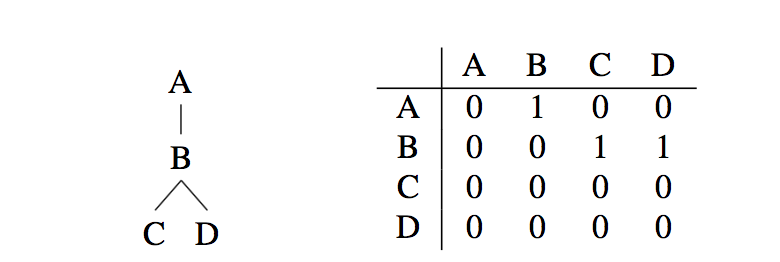
\includegraphics[width=6cm]{./figs/graph-matrix.png}
	\caption{4-graph example: Element of adjacency matrix is a binary string ``0100 0011 0000 0000", for which the decimal number is 17152}
	\label{fig:graph-ex}
	\end{figure}

	\item \textbf{Library Calls} \\
	If call of any contract from any other library occurs in the contract, addresses of all library contracts will be recorded. Similarity among them will be calculated with Jacobian similarity formula.

	\item \textbf{Type Signature} \\
	This feature is composed of input parameter type and return parameter type, and similarity between them can be calculated with Jacobian similarity formula. For example, for the following smart contract code, feature of Type Signature of function ``getBalance" is vector (address, uint256). \\

	\begin{figure}[h]
  	\centering
  	\begin{minipage}{.7\linewidth}
	\begin{lstlisting}[frame=single]
contract addressTest {
  function getBalance(address addr) returns (uint) {
  	return addr.balance;
  }
}
	\end{lstlisting}
  	\end{minipage}
	\end{figure}

	\item \textbf{Local Types:} This feature is the set of all types of local variables of the function body, for which similarity should be calculated with Jacobian similarity formula.

	\item \textbf{Numeric Literals:} The set of all numeric constants serves as the feature of Numeric Literals, for which similarity should be calculated with Jacobian similarity formula.

	\item \textbf{String Literals:} The set of all string constants serves as the feature of String Literals, for which similarity should be calculated with Jacobian similarity formula.
\end{itemize}

Feature family can be expanded, so it is convenient to add new features to it. Based on the circumstance that there is a similarity calculation for each feature, we calculate the weighted sum of all features and thus can acquire the final code similarity:

\begin{equation}
	sim_{combined}(\vec{A}, \vec{B})=\frac{\sum_{c=1}^{n_{cl}}sim_{c}(\vec{A_c},~\vec{B_c})\cdot w_{c}}{\sum_{c=1}^{n_{cl}}w_{c}}
\end{equation}

Therein, $\vec{A}$ and $\vec{B}$ are eigenvectors; $n_{cl}$ is number of features in the feature family; $sim_{c}$ is similarity calculation function specific to feature c; $\vec{A_c}$ and $\vec{B_c}$ are eigenvectors of feature c; $w_{c}$ is weight of c. Weight can be acquired through machine learning algorithm training based on a large number of test sets.